
\section{MARKET LANDSCAPE} \label{landscape}
During 2016 alone, an estimated 1.61 billion people purchased goods online and global e-retail sales amounted to \$1.9trillion. In Asia Pacific, online sales accounted for 12.1\% of retail sales, but only 1.8\% in the Middle East and Africa. Projections on market growth, estimate a growth of up to \$4.06trillion by 2020. These projections are based on global buying trends driven by millennials, on  GDP forecasts  driven by certain geographies and web-related industries, growth on emerging markets such as Africa, predicting a large number of new internet users added to the global market pool, becoming decisive for future online sales.
 
Global statistics reveal that purchase intention rates among online shoppers vary strongly by product category - as we can see in Figure \ref{fig:file_categories}, 50\% of online purchases involve books (hard copies \& eBooks) and music . The average number of annual online transactions per capita is not uniform - Asian buyers account for an average of 22.1\% of online transactions, whereas buyers in Latin America represent a 9.2\%. 

The online digital files market is rapidly expanding and as we can see in Figure \ref{fig:market}, it is expected to double in size over the next two years. As the market expands, a multitude of distribution channels exist for creators to sell their digital content. 

\begin{figure}[!bp]
\centering
\begin{minipage}{.5\textwidth}
  \centering
  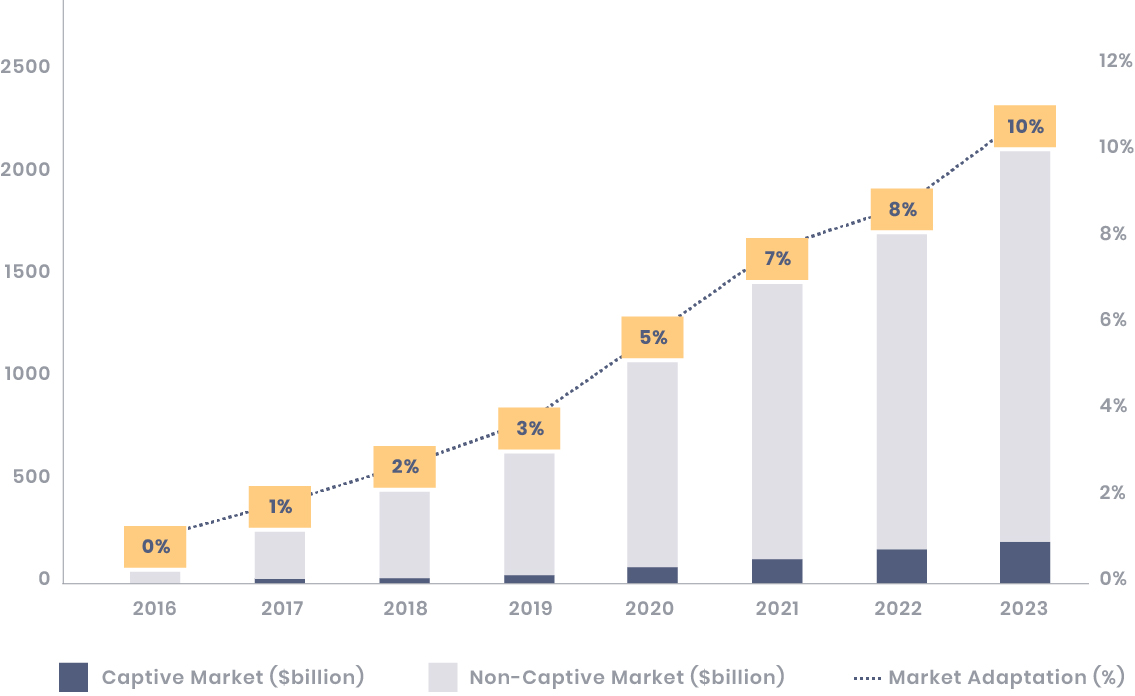
\includegraphics[width=0.8\linewidth]{./figures/fig1.jpg}
  \captionof{figure}{Online digital files market ( \$billion )}
  \label{fig:market}
\end{minipage}%
\begin{minipage}{.5\textwidth}
  \centering
  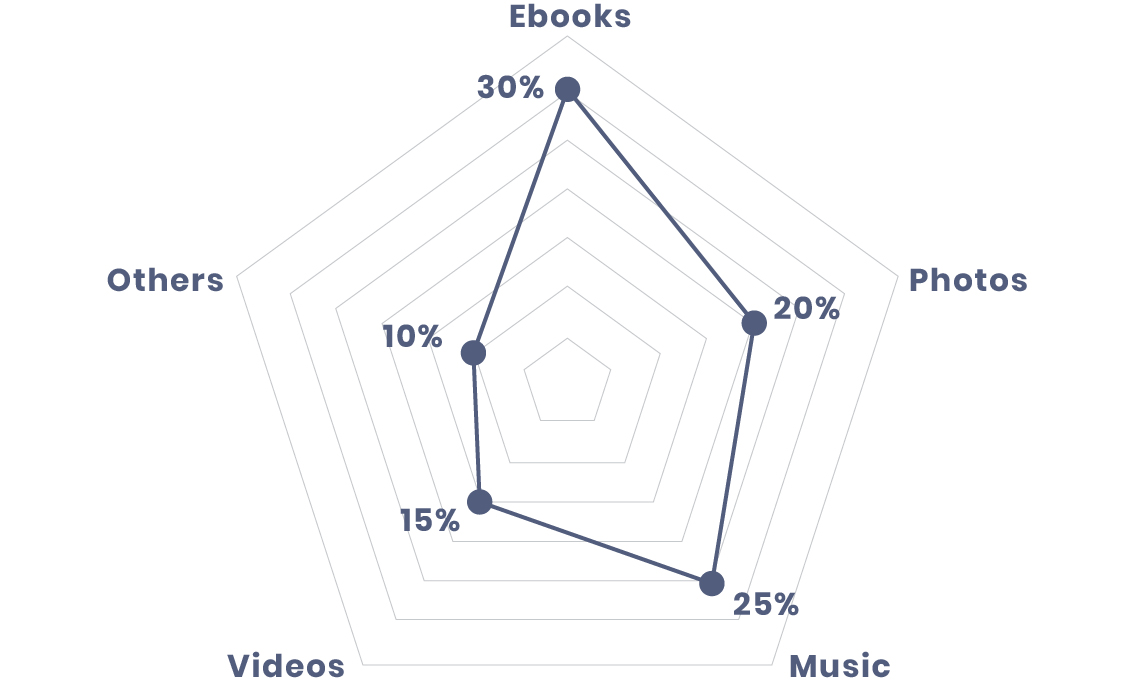
\includegraphics[width=0.8\linewidth]{./figures/fig2.jpg}
  \captionof{figure}{Digital file categories sales}
  \label{fig:file_categories}
\end{minipage} 
\end{figure}


The main distinction among current offerings is whether the solution used facilitates a direct connection between the creator and the buyer or it enables the creator to reach a wider audience without facilitating a direct sell. Using industry terms, the two main offerings are known as Maker Platforms and Exchange Platforms and in the following section we will review their advantages and shortcomings.
The online digital files market is rapidly expanding and as we can see in Figure \ref{fig:market}, it is expected to double in size over the next two years. Among the types of files that are sold online, Ebooks and music account for over 50\% of the sales ( Figure \ref{fig:file_categories} ). 
 


%%%%%%%%%%%%%%%%%%%%%%%%%%%%%%%%%%%%%%%%%%%%%%%%%%%%%%%%%%%%%%%%%%%%%%
\subsection{Maker Platforms}

Several stock content websites exist where creators can fully give up their licensing and pricing rights and get a commission on copies of work sold. Such websites do not require a subscription by the creator but are customer centric and provide subscription plans for end users. Submitted work needs to go through a thorough vetting process before it is included in the catalog of works available. Such websites theoretically offer a lot of visibility since they tend to have a huge user base but, in practice, ones work can easily be lost among the myriad of similar offerings. As we can see in Table \ref{comp-matrix} creators only receive a small fraction of the retail price of their work, buyers need to have a valid paid subscription and creators have no control over the licensing and pricing of their work.


%%%%%%%%%%%%%%%%%%%%%%%%%%%%%%%%%%%%%%%%%%%%%%%%%%%%%%%%%%%%%%%%%%%%%%

\subsection{Exchange Platforms}

Exchange platforms enable creators to facilitate a direct sell by providing an inventory, payment processing, shopping cart and cloud based storage as a service. Such offerings usually require a time-based subscription by the creator and display product listings either in a central website or provide embeddable widgets that creators can use to display and sell their products through their own website. While Exchange Platforms give full control to creators over the licensing and pricing of their work, as we can see in Table \ref{comp-matrix} they are charged a fee on work sold and an active paid subscription is required.
\newline
\bigskip

\subsection{BUSINESS MODEL} \label{businessmodel}

Both solutions as described above, have a centralized nature and impose great restrictions to Creators and Buyers.

BlockLicense introduces a new business model that puts Creators and Buyers at the forefront by removing all restrictions imposed by Maker and Exchange Platforms and by  providing tools that simplify the licensing process and allow a wide range of licensing scenarios. Payment processing and routing as well as proof-of-ownership is automated with Ethereum smart contracts.

Multiple channels of distribution are provided including a Web Platform, website embedded shops \& offline distribution of files. All transactions and payouts within BlockLicense are instant while both creators and buyers are free of subscription or hidden costs. A flat 2\% fee is imposed in all transactions to cover BlockLicense costs and allow a continuous and organic expansion of the ecosystem.

\begin{figure}[bp]
\centering
\begin{minipage}{.45\textwidth}
  \centering
  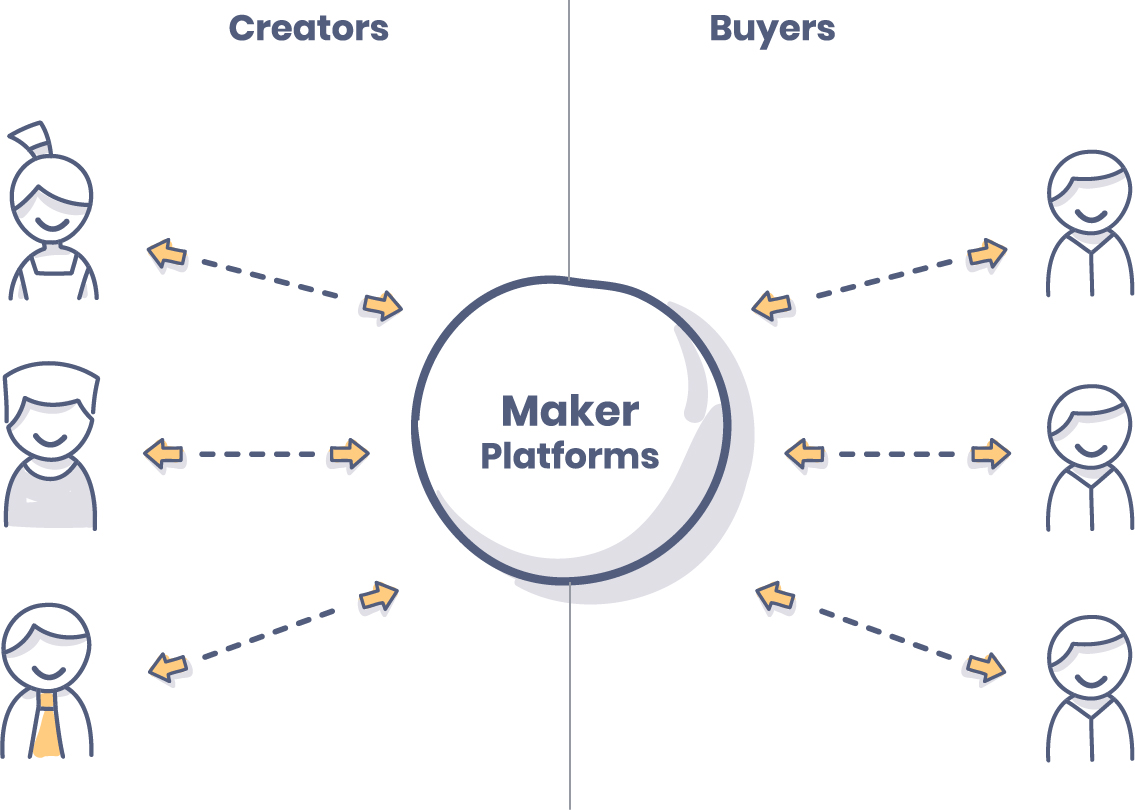
\includegraphics[width=.8\linewidth]{./figures/fig9.jpg}
  \captionof{figure}{Maker Platforms.}
  \label{fig:maker}
\end{minipage}
\begin{minipage}{.45\textwidth}
  \centering
  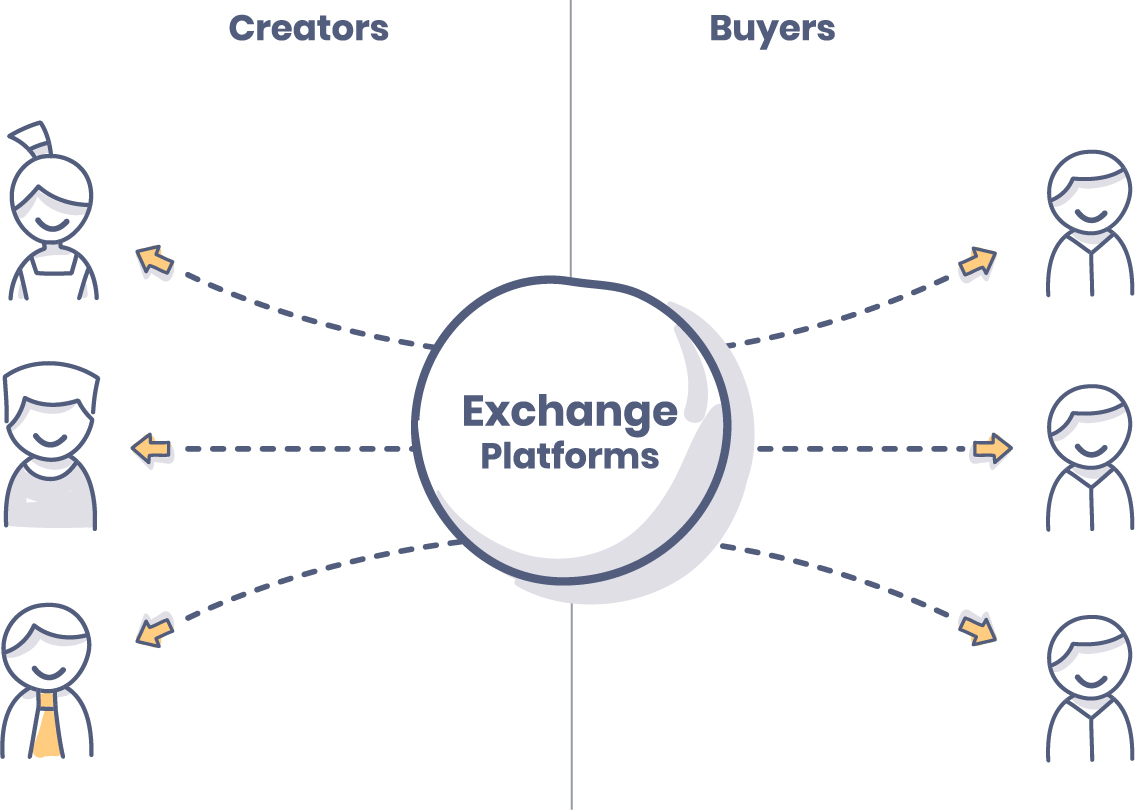
\includegraphics[width=.8\linewidth]{./figures/fig10.jpg}
  \captionof{figure}{Exchange Platforms.}
  \label{fig:exchange}
\end{minipage}%
\end{figure}
